\documentclass[]{article}
\usepackage{lmodern}
\usepackage{amssymb,amsmath}
\usepackage{ifxetex,ifluatex}
\usepackage{fixltx2e} % provides \textsubscript
\ifnum 0\ifxetex 1\fi\ifluatex 1\fi=0 % if pdftex
  \usepackage[T1]{fontenc}
  \usepackage[utf8]{inputenc}
\else % if luatex or xelatex
  \ifxetex
    \usepackage{mathspec}
  \else
    \usepackage{fontspec}
  \fi
  \defaultfontfeatures{Ligatures=TeX,Scale=MatchLowercase}
\fi
% use upquote if available, for straight quotes in verbatim environments
\IfFileExists{upquote.sty}{\usepackage{upquote}}{}
% use microtype if available
\IfFileExists{microtype.sty}{%
\usepackage{microtype}
\UseMicrotypeSet[protrusion]{basicmath} % disable protrusion for tt fonts
}{}
\usepackage[margin=1in]{geometry}
\usepackage{hyperref}
\hypersetup{unicode=true,
            pdftitle={Assignment \#4},
            pdfauthor={Peyman Kor},
            pdfborder={0 0 0},
            breaklinks=true}
\urlstyle{same}  % don't use monospace font for urls
\usepackage{color}
\usepackage{fancyvrb}
\newcommand{\VerbBar}{|}
\newcommand{\VERB}{\Verb[commandchars=\\\{\}]}
\DefineVerbatimEnvironment{Highlighting}{Verbatim}{commandchars=\\\{\}}
% Add ',fontsize=\small' for more characters per line
\usepackage{framed}
\definecolor{shadecolor}{RGB}{248,248,248}
\newenvironment{Shaded}{\begin{snugshade}}{\end{snugshade}}
\newcommand{\AlertTok}[1]{\textcolor[rgb]{0.94,0.16,0.16}{#1}}
\newcommand{\AnnotationTok}[1]{\textcolor[rgb]{0.56,0.35,0.01}{\textbf{\textit{#1}}}}
\newcommand{\AttributeTok}[1]{\textcolor[rgb]{0.77,0.63,0.00}{#1}}
\newcommand{\BaseNTok}[1]{\textcolor[rgb]{0.00,0.00,0.81}{#1}}
\newcommand{\BuiltInTok}[1]{#1}
\newcommand{\CharTok}[1]{\textcolor[rgb]{0.31,0.60,0.02}{#1}}
\newcommand{\CommentTok}[1]{\textcolor[rgb]{0.56,0.35,0.01}{\textit{#1}}}
\newcommand{\CommentVarTok}[1]{\textcolor[rgb]{0.56,0.35,0.01}{\textbf{\textit{#1}}}}
\newcommand{\ConstantTok}[1]{\textcolor[rgb]{0.00,0.00,0.00}{#1}}
\newcommand{\ControlFlowTok}[1]{\textcolor[rgb]{0.13,0.29,0.53}{\textbf{#1}}}
\newcommand{\DataTypeTok}[1]{\textcolor[rgb]{0.13,0.29,0.53}{#1}}
\newcommand{\DecValTok}[1]{\textcolor[rgb]{0.00,0.00,0.81}{#1}}
\newcommand{\DocumentationTok}[1]{\textcolor[rgb]{0.56,0.35,0.01}{\textbf{\textit{#1}}}}
\newcommand{\ErrorTok}[1]{\textcolor[rgb]{0.64,0.00,0.00}{\textbf{#1}}}
\newcommand{\ExtensionTok}[1]{#1}
\newcommand{\FloatTok}[1]{\textcolor[rgb]{0.00,0.00,0.81}{#1}}
\newcommand{\FunctionTok}[1]{\textcolor[rgb]{0.00,0.00,0.00}{#1}}
\newcommand{\ImportTok}[1]{#1}
\newcommand{\InformationTok}[1]{\textcolor[rgb]{0.56,0.35,0.01}{\textbf{\textit{#1}}}}
\newcommand{\KeywordTok}[1]{\textcolor[rgb]{0.13,0.29,0.53}{\textbf{#1}}}
\newcommand{\NormalTok}[1]{#1}
\newcommand{\OperatorTok}[1]{\textcolor[rgb]{0.81,0.36,0.00}{\textbf{#1}}}
\newcommand{\OtherTok}[1]{\textcolor[rgb]{0.56,0.35,0.01}{#1}}
\newcommand{\PreprocessorTok}[1]{\textcolor[rgb]{0.56,0.35,0.01}{\textit{#1}}}
\newcommand{\RegionMarkerTok}[1]{#1}
\newcommand{\SpecialCharTok}[1]{\textcolor[rgb]{0.00,0.00,0.00}{#1}}
\newcommand{\SpecialStringTok}[1]{\textcolor[rgb]{0.31,0.60,0.02}{#1}}
\newcommand{\StringTok}[1]{\textcolor[rgb]{0.31,0.60,0.02}{#1}}
\newcommand{\VariableTok}[1]{\textcolor[rgb]{0.00,0.00,0.00}{#1}}
\newcommand{\VerbatimStringTok}[1]{\textcolor[rgb]{0.31,0.60,0.02}{#1}}
\newcommand{\WarningTok}[1]{\textcolor[rgb]{0.56,0.35,0.01}{\textbf{\textit{#1}}}}
\usepackage{graphicx,grffile}
\makeatletter
\def\maxwidth{\ifdim\Gin@nat@width>\linewidth\linewidth\else\Gin@nat@width\fi}
\def\maxheight{\ifdim\Gin@nat@height>\textheight\textheight\else\Gin@nat@height\fi}
\makeatother
% Scale images if necessary, so that they will not overflow the page
% margins by default, and it is still possible to overwrite the defaults
% using explicit options in \includegraphics[width, height, ...]{}
\setkeys{Gin}{width=\maxwidth,height=\maxheight,keepaspectratio}
\IfFileExists{parskip.sty}{%
\usepackage{parskip}
}{% else
\setlength{\parindent}{0pt}
\setlength{\parskip}{6pt plus 2pt minus 1pt}
}
\setlength{\emergencystretch}{3em}  % prevent overfull lines
\providecommand{\tightlist}{%
  \setlength{\itemsep}{0pt}\setlength{\parskip}{0pt}}
\setcounter{secnumdepth}{0}
% Redefines (sub)paragraphs to behave more like sections
\ifx\paragraph\undefined\else
\let\oldparagraph\paragraph
\renewcommand{\paragraph}[1]{\oldparagraph{#1}\mbox{}}
\fi
\ifx\subparagraph\undefined\else
\let\oldsubparagraph\subparagraph
\renewcommand{\subparagraph}[1]{\oldsubparagraph{#1}\mbox{}}
\fi

%%% Use protect on footnotes to avoid problems with footnotes in titles
\let\rmarkdownfootnote\footnote%
\def\footnote{\protect\rmarkdownfootnote}

%%% Change title format to be more compact
\usepackage{titling}

% Create subtitle command for use in maketitle
\providecommand{\subtitle}[1]{
  \posttitle{
    \begin{center}\large#1\end{center}
    }
}

\setlength{\droptitle}{-2em}

  \title{Assignment \#4}
    \pretitle{\vspace{\droptitle}\centering\huge}
  \posttitle{\par}
    \author{Peyman Kor}
    \preauthor{\centering\large\emph}
  \postauthor{\par}
      \predate{\centering\large\emph}
  \postdate{\par}
    \date{11/28/2019}


\begin{document}
\maketitle

\#4.1

\begin{Shaded}
\begin{Highlighting}[]
\KeywordTok{library}\NormalTok{(tidyverse)}
\end{Highlighting}
\end{Shaded}

\begin{verbatim}
## -- Attaching packages ------------------------------------------------------------------------------------- tidyverse 1.2.1 --
\end{verbatim}

\begin{verbatim}
## v ggplot2 3.2.1     v purrr   0.3.2
## v tibble  2.1.3     v dplyr   0.8.3
## v tidyr   0.8.3     v stringr 1.4.0
## v readr   1.3.1     v forcats 0.4.0
\end{verbatim}

\begin{verbatim}
## -- Conflicts ---------------------------------------------------------------------------------------- tidyverse_conflicts() --
## x dplyr::filter() masks stats::filter()
## x dplyr::lag()    masks stats::lag()
\end{verbatim}

\begin{Shaded}
\begin{Highlighting}[]
\NormalTok{data <-}\StringTok{ }\KeywordTok{read.csv}\NormalTok{(}\StringTok{'A4_Kulhuse.csv'}\NormalTok{)}
\KeywordTok{head}\NormalTok{(data)}
\end{Highlighting}
\end{Shaded}

\begin{verbatim}
##    Temp   Sal Depth   pH  Chl ODOsat  ODO Battery            DateTime
## 1 18.22 18.03 5.191 8.25 2.91  108.6 9.19    12.7 2017-08-24 10:00:00
## 2 18.30 17.96 5.213 8.26 4.11  107.7 9.10    12.7 2017-08-24 10:30:00
## 3 18.29 18.00 5.234 8.26 4.01  108.5 9.17    12.7 2017-08-24 11:00:00
## 4 18.30 18.00 5.258 8.26 4.33  108.8 9.20    12.7 2017-08-24 11:30:00
## 5 18.34 18.02 5.277 8.26 3.74  110.1 9.29    12.7 2017-08-24 12:00:00
## 6 18.35 18.04 5.282 8.26 4.45  110.9 9.36    12.7 2017-08-24 12:30:00
\end{verbatim}

Now, let's have alook on the data for possible ``NA'' values,

\begin{Shaded}
\begin{Highlighting}[]
\NormalTok{data_fil <-}\StringTok{ }\NormalTok{data }\OperatorTok\StringTok{ }\KeywordTok{filter}\NormalTok{(}\KeywordTok{is.na}\NormalTok{(Sal))}
\end{Highlighting}
\end{Shaded}

We see that the column Salinity has 111 rows whcih are NA, also we could
see other columns as well are NA, so could safely removes these 111 rows
beacuse they contain no information.

\begin{Shaded}
\begin{Highlighting}[]
\NormalTok{data_nona <-}\StringTok{ }\NormalTok{data }\OperatorTok\StringTok{ }\KeywordTok{filter}\NormalTok{(}\OperatorTok{!}\KeywordTok{is.na}\NormalTok{(Sal))}
\end{Highlighting}
\end{Shaded}

Having this now, we visulize the Salinity versus time:

\begin{Shaded}
\begin{Highlighting}[]
\KeywordTok{library}\NormalTok{(ggplot2)}
\NormalTok{data_nona }\OperatorTok\StringTok{ }\KeywordTok{mutate}\NormalTok{(}\DataTypeTok{Date =} \KeywordTok{as.Date}\NormalTok{(DateTime)) }\OperatorTok\StringTok{ }
\StringTok{  }\KeywordTok{ggplot}\NormalTok{(}\DataTypeTok{mapping =} \KeywordTok{aes}\NormalTok{(Date,Sal)) }\OperatorTok{+}
\StringTok{  }\KeywordTok{geom_point}\NormalTok{() }\OperatorTok{+}
\StringTok{  }\KeywordTok{scale_x_date}\NormalTok{(}\DataTypeTok{date_minor_breaks =} \StringTok{"1 day "}\NormalTok{,}\DataTypeTok{date_labels =} \StringTok{"%b %d"}\NormalTok{) }\OperatorTok{+}
\StringTok{  }\KeywordTok{stat_smooth}\NormalTok{(}
  \DataTypeTok{color =} \StringTok{"#FC4E07"}\NormalTok{,}
  \DataTypeTok{method =} \StringTok{"loess"}
\NormalTok{  )}
\end{Highlighting}
\end{Shaded}

\includegraphics{Assignment-4_files/figure-latex/unnamed-chunk-4-1.pdf}

\begin{Shaded}
\begin{Highlighting}[]
\KeywordTok{library}\NormalTok{(ggplot2)}
\NormalTok{data_nona }\OperatorTok\StringTok{ }\KeywordTok{mutate}\NormalTok{(}\DataTypeTok{Date =} \KeywordTok{as.Date}\NormalTok{(DateTime)) }\OperatorTok\StringTok{ }
\StringTok{  }\KeywordTok{ggplot}\NormalTok{(}\DataTypeTok{mapping =} \KeywordTok{aes}\NormalTok{(Date,ODO)) }\OperatorTok{+}
\StringTok{  }\KeywordTok{geom_point}\NormalTok{() }\OperatorTok{+}
\StringTok{  }\KeywordTok{scale_x_date}\NormalTok{(}\DataTypeTok{date_minor_breaks =} \StringTok{"1 day "}\NormalTok{,}\DataTypeTok{date_labels =} \StringTok{"%b %d"}\NormalTok{) }\OperatorTok{+}
\StringTok{  }\KeywordTok{stat_smooth}\NormalTok{(}
  \DataTypeTok{color =} \StringTok{"#FC4E07"}\NormalTok{,}
  \DataTypeTok{method =} \StringTok{"loess"}
\NormalTok{  )}
\end{Highlighting}
\end{Shaded}

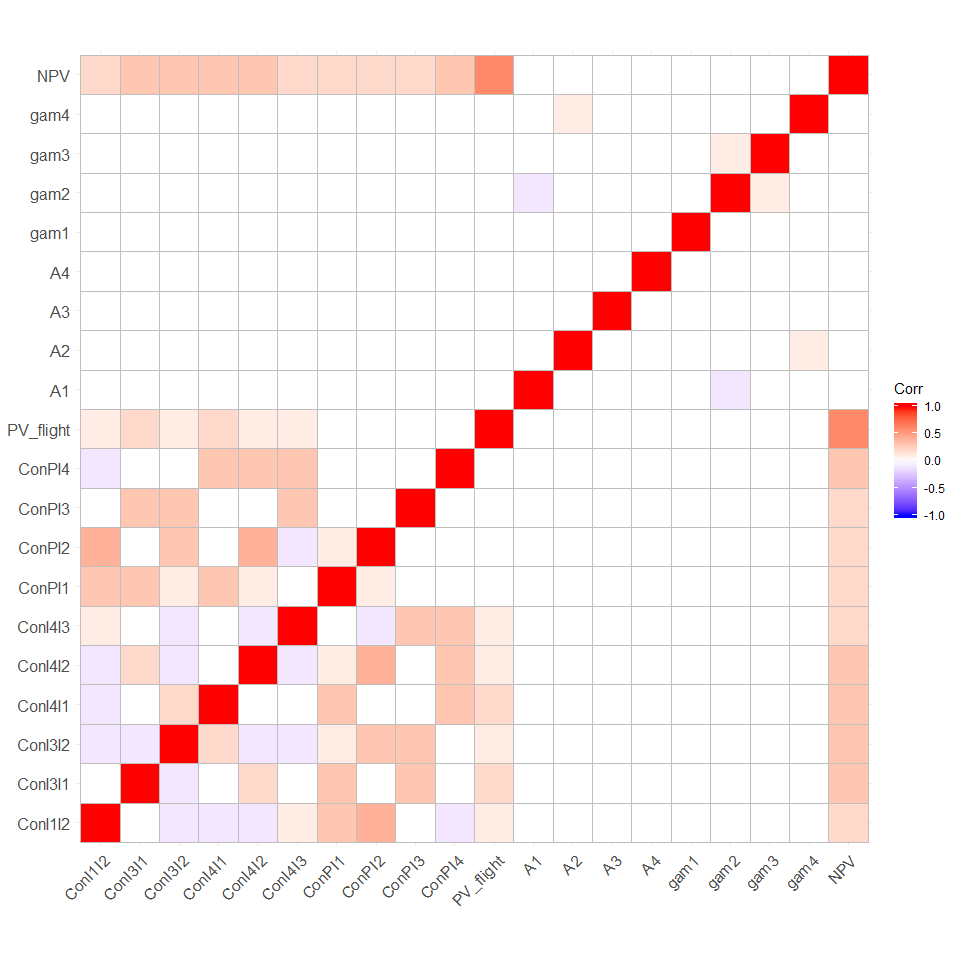
\includegraphics{Assignment-4_files/figure-latex/unnamed-chunk-5-1.pdf}

\hypertarget{section}{%
\section{4.2}\label{section}}

The salinity assumed to be random walk process as the follow:

\[X_{t} = X_{t-1} + \eta_{t}\] \[Y_{t} = X_{t} + \epsilon_{t}\]

So, the following is the state space model for salinity, where the
\(\eta_{t}\) and \(\epsilon_{t}\) are the white noise with the standard
deviation of \(\sigma_{\eta}\) and \(\sigma_{\epsilon}\).

On the other hand, the salinity could be written as the ARIMA process
(0,1,1) as the follow:

\[Y_{t}-Y_{t-1} = \eta_{t} + \epsilon_{t}-\epsilon_{t-1}\]

In the state space model as the matrix,

\[X_t=AX_{t-1} + G\epsilon_{t}\] \[Y =CX_t\]

Where the \(A=C=1\)

\hypertarget{section-1}{%
\section{4.3}\label{section-1}}

\begin{Shaded}
\begin{Highlighting}[]
\KeywordTok{library}\NormalTok{(FKF)}
\end{Highlighting}
\end{Shaded}

\begin{verbatim}
## Loading required package: RUnit
\end{verbatim}

\begin{Shaded}
\begin{Highlighting}[]
\NormalTok{y <-}\StringTok{ }\NormalTok{data_nona}\OperatorTok{$}\NormalTok{Sal}
\NormalTok{dt <-}\StringTok{ }\NormalTok{ct <-}\StringTok{ }\KeywordTok{matrix}\NormalTok{(}\DecValTok{0}\NormalTok{)}
\NormalTok{Zt <-}\StringTok{ }\NormalTok{Tt <-}\StringTok{ }\KeywordTok{matrix}\NormalTok{(}\DecValTok{1}\NormalTok{)}
\NormalTok{a0 <-}\StringTok{ }\NormalTok{y[}\DecValTok{1}\NormalTok{] }\CommentTok{# Estimation of the first year flow}
\NormalTok{P0 <-}\StringTok{ }\KeywordTok{matrix}\NormalTok{(}\FloatTok{0.01}\NormalTok{) }\CommentTok{# Variance of 'a0'}
\NormalTok{fit.fkf <-}\StringTok{ }\KeywordTok{optim}\NormalTok{(}\KeywordTok{c}\NormalTok{(}\DataTypeTok{HHt =} \FloatTok{0.01}\NormalTok{ ,}
                   \DataTypeTok{GGt =} \FloatTok{0.005}\NormalTok{ ),}
                 \DataTypeTok{fn =} \ControlFlowTok{function}\NormalTok{(par, ...)}
                   \OperatorTok{-}\KeywordTok{fkf}\NormalTok{(}\DataTypeTok{HHt =} \KeywordTok{matrix}\NormalTok{(par[}\DecValTok{1}\NormalTok{]), }\DataTypeTok{GGt =} \KeywordTok{matrix}\NormalTok{(par[}\DecValTok{2}\NormalTok{]), ...)}\OperatorTok{$}\NormalTok{logLik,}
                 \DataTypeTok{yt =} \KeywordTok{rbind}\NormalTok{(y), }\DataTypeTok{a0 =}\NormalTok{ a0, }\DataTypeTok{P0 =}\NormalTok{ P0, }\DataTypeTok{dt =}\NormalTok{ dt, }\DataTypeTok{ct =}\NormalTok{ ct,}
                 \DataTypeTok{Zt =}\NormalTok{ Zt, }\DataTypeTok{Tt =}\NormalTok{ Tt)}
\CommentTok{## Filter Nile data with estimated parameters:plot.fkf 7}
\NormalTok{fkf.obj <-}\StringTok{ }\KeywordTok{fkf}\NormalTok{(a0, P0, dt, ct, Tt, Zt, }\DataTypeTok{HHt =} \KeywordTok{matrix}\NormalTok{(fit.fkf}\OperatorTok{$}\NormalTok{par[}\DecValTok{1}\NormalTok{]),}
               \DataTypeTok{GGt =} \KeywordTok{matrix}\NormalTok{(fit.fkf}\OperatorTok{$}\NormalTok{par[}\DecValTok{2}\NormalTok{]), }\DataTypeTok{yt =} \KeywordTok{rbind}\NormalTok{(y))}
\end{Highlighting}
\end{Shaded}

\begin{Shaded}
\begin{Highlighting}[]
\KeywordTok{plot}\NormalTok{(y)}
\KeywordTok{with}\NormalTok{(fkf.obj, }\KeywordTok{matlines}\NormalTok{((at[}\DecValTok{1}\NormalTok{,]) }\OperatorTok{+}\StringTok{ }\KeywordTok{cbind}\NormalTok{(}\DecValTok{0}\NormalTok{,}\OperatorTok{-}\FloatTok{1.96}\OperatorTok{*}\KeywordTok{sqrt}\NormalTok{(Pt[}\DecValTok{1}\NormalTok{,}\DecValTok{1}\NormalTok{,]),}\FloatTok{1.96}\OperatorTok{*}\KeywordTok{sqrt}\NormalTok{(Pt[}\DecValTok{1}\NormalTok{,}\DecValTok{1}\NormalTok{,])),}\DataTypeTok{type=}\StringTok{"l"}\NormalTok{, }\DataTypeTok{lty=}\KeywordTok{c}\NormalTok{(}\DecValTok{1}\NormalTok{,}\DecValTok{2}\NormalTok{,}\DecValTok{2}\NormalTok{), }\DataTypeTok{col=}\DecValTok{2}\NormalTok{))}
\KeywordTok{legend}\NormalTok{(}\StringTok{"bottom"}\NormalTok{, }\KeywordTok{c}\NormalTok{(}\StringTok{"Salinity Data"}\NormalTok{, }\StringTok{"Estimation and Confidence Interval"}\NormalTok{),}
       \DataTypeTok{col =} \KeywordTok{c}\NormalTok{(}\StringTok{"black"}\NormalTok{, }\StringTok{"red"}\NormalTok{), }\DataTypeTok{lty =} \DecValTok{1}\NormalTok{)}
\end{Highlighting}
\end{Shaded}

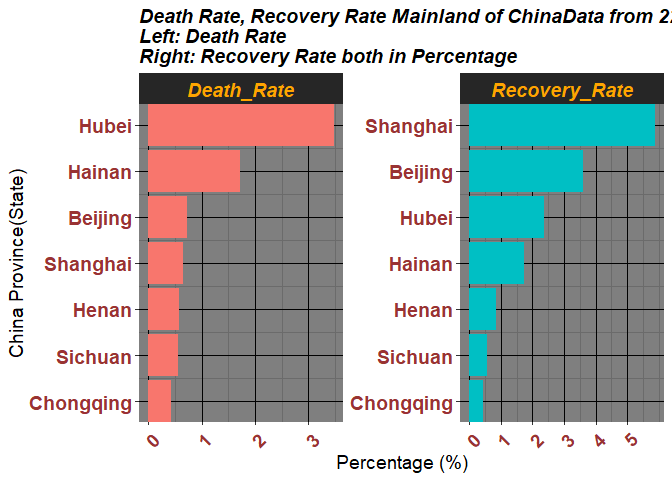
\includegraphics{Assignment-4_files/figure-latex/unnamed-chunk-7-1.pdf}

\begin{Shaded}
\begin{Highlighting}[]
\KeywordTok{plot}\NormalTok{(y, }\DataTypeTok{main =} \StringTok{"Treering data"}\NormalTok{)}
\KeywordTok{lines}\NormalTok{(}\KeywordTok{ts}\NormalTok{(fkf.obj}\OperatorTok{$}\NormalTok{att[}\DecValTok{1}\NormalTok{, ], }\DataTypeTok{start =} \KeywordTok{start}\NormalTok{(y), }\DataTypeTok{frequency =} \KeywordTok{frequency}\NormalTok{(y)), }\DataTypeTok{col =} \StringTok{"blue"}\NormalTok{)}
\end{Highlighting}
\end{Shaded}

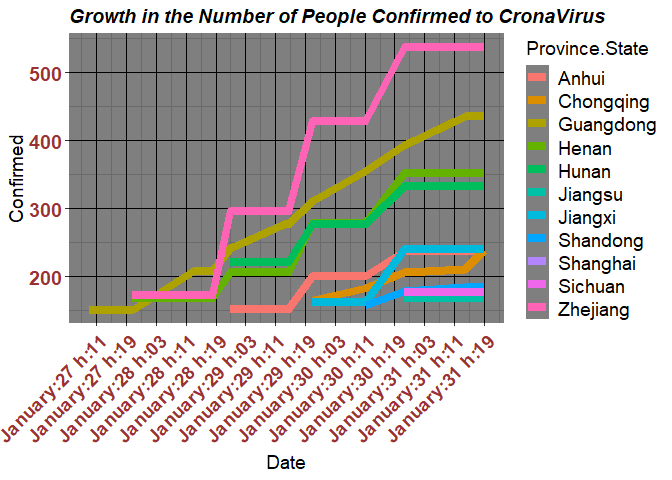
\includegraphics{Assignment-4_files/figure-latex/unnamed-chunk-8-1.pdf}

\begin{Shaded}
\begin{Highlighting}[]
\NormalTok{prediction <-}\StringTok{ }\NormalTok{fkf.obj}\OperatorTok{$}\NormalTok{att[}\DecValTok{1}\NormalTok{, ]}
\NormalTok{error <-}\StringTok{ }\KeywordTok{abs}\NormalTok{(y}\OperatorTok{-}\NormalTok{prediction)}
\NormalTok{norm_err <-}\StringTok{ }\NormalTok{error}\OperatorTok{/}\KeywordTok{sd}\NormalTok{(prediction)}
\KeywordTok{plot}\NormalTok{(norm_err)}
\end{Highlighting}
\end{Shaded}

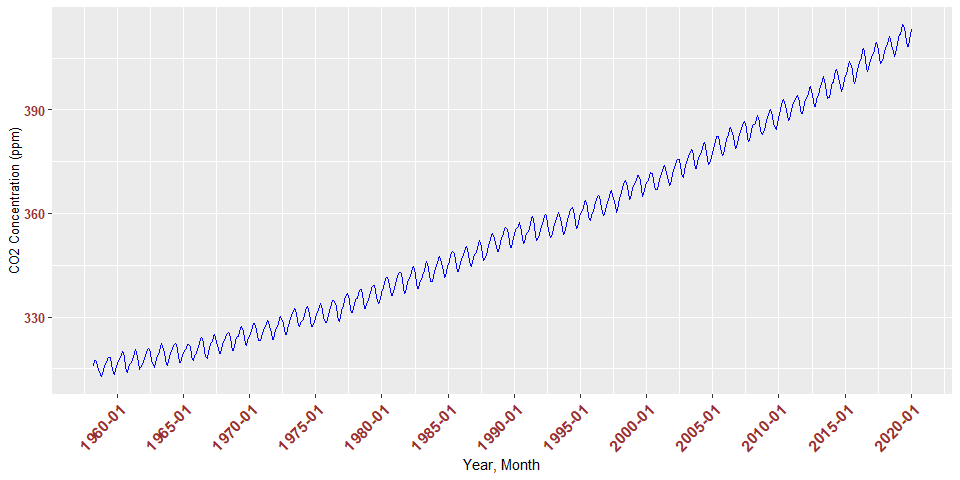
\includegraphics{Assignment-4_files/figure-latex/unnamed-chunk-9-1.pdf}

\begin{Shaded}
\begin{Highlighting}[]
\KeywordTok{plot}\NormalTok{(y[}\DecValTok{800}\OperatorTok{:}\DecValTok{950}\NormalTok{], }\DataTypeTok{main =} \StringTok{"Treering data"}\NormalTok{)}
\KeywordTok{lines}\NormalTok{(}\KeywordTok{ts}\NormalTok{(fkf.obj}\OperatorTok{$}\NormalTok{att[}\DecValTok{1}\NormalTok{, ][}\DecValTok{800}\OperatorTok{:}\DecValTok{950}\NormalTok{], }\DataTypeTok{start =} \KeywordTok{start}\NormalTok{(y), }\DataTypeTok{frequency =} \KeywordTok{frequency}\NormalTok{(y)), }\DataTypeTok{col =} \StringTok{"blue"}\NormalTok{)}
\end{Highlighting}
\end{Shaded}

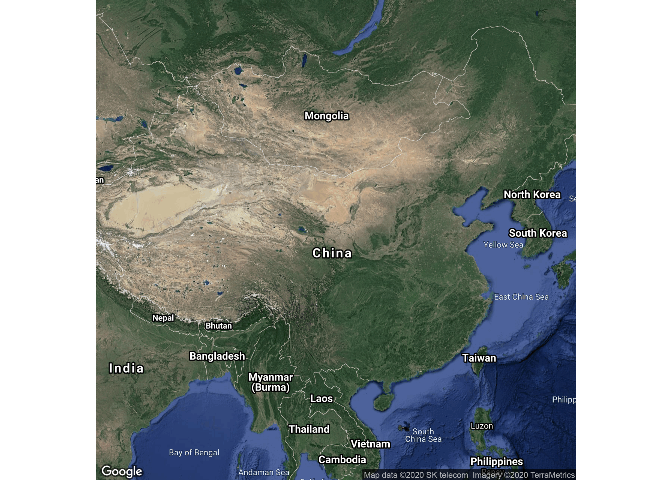
\includegraphics{Assignment-4_files/figure-latex/unnamed-chunk-10-1.pdf}

\begin{Shaded}
\begin{Highlighting}[]
\NormalTok{prediction <-}\StringTok{ }\NormalTok{fkf.obj}\OperatorTok{$}\NormalTok{att[}\DecValTok{1}\NormalTok{, ]}
\NormalTok{error <-}\StringTok{ }\KeywordTok{abs}\NormalTok{(y}\OperatorTok{-}\NormalTok{prediction)}
\NormalTok{norm_err <-}\StringTok{ }\NormalTok{error}\OperatorTok{/}\KeywordTok{sd}\NormalTok{(prediction)}
\KeywordTok{plot}\NormalTok{(norm_err[}\DecValTok{800}\OperatorTok{:}\DecValTok{950}\NormalTok{])}
\end{Highlighting}
\end{Shaded}

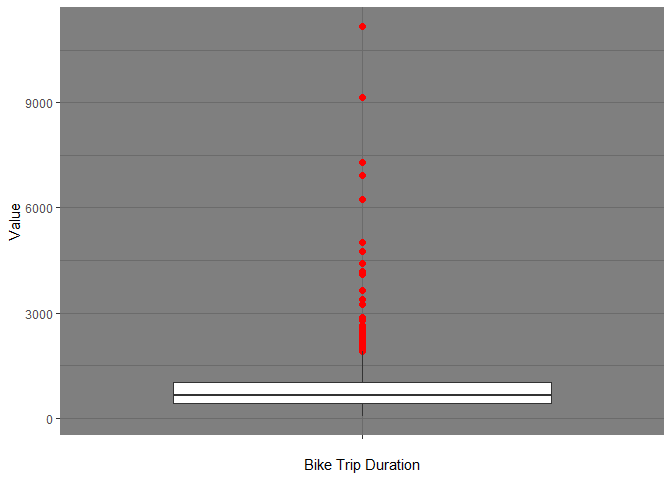
\includegraphics{Assignment-4_files/figure-latex/unnamed-chunk-11-1.pdf}

\begin{Shaded}
\begin{Highlighting}[]
\NormalTok{prediction[}\DecValTok{4889}\NormalTok{]}
\end{Highlighting}
\end{Shaded}

\begin{verbatim}
## [1] 20.69859
\end{verbatim}

\hypertarget{section-2}{%
\section{4}\label{section-2}}

\begin{Shaded}
\begin{Highlighting}[]
\NormalTok{sd_pre <-}\StringTok{ }\KeywordTok{sd}\NormalTok{(prediction)}
\KeywordTok{sum}\NormalTok{(}\KeywordTok{abs}\NormalTok{(prediction}\OperatorTok{-}\NormalTok{y) }\OperatorTok{>}\StringTok{ }\DecValTok{6}\OperatorTok{*}\NormalTok{sd_pre)}
\end{Highlighting}
\end{Shaded}

\begin{verbatim}
## [1] 6
\end{verbatim}

\hypertarget{section-3}{%
\section{5}\label{section-3}}

\begin{Shaded}
\begin{Highlighting}[]
\NormalTok{y <-}\StringTok{ }\NormalTok{data_nona}\OperatorTok{$}\NormalTok{Sal[}\DecValTok{1}\OperatorTok{:}\DecValTok{800}\NormalTok{]}
\NormalTok{dt <-}\StringTok{ }\NormalTok{ct <-}\StringTok{ }\KeywordTok{matrix}\NormalTok{(}\DecValTok{0}\NormalTok{)}
\NormalTok{Zt <-}\StringTok{ }\NormalTok{Tt <-}\StringTok{ }\KeywordTok{matrix}\NormalTok{(}\DecValTok{1}\NormalTok{)}
\NormalTok{a0 <-}\StringTok{ }\NormalTok{y[}\DecValTok{1}\NormalTok{] }\CommentTok{# Estimation of the first year flow}
\NormalTok{P0 <-}\StringTok{ }\KeywordTok{matrix}\NormalTok{(}\FloatTok{0.01}\NormalTok{) }\CommentTok{# Variance of 'a0'}
\NormalTok{fit.fkf <-}\StringTok{ }\KeywordTok{optim}\NormalTok{(}\KeywordTok{c}\NormalTok{(}\DataTypeTok{HHt =} \FloatTok{0.0}\NormalTok{ ,}
                   \DataTypeTok{GGt =} \FloatTok{0.005}\NormalTok{ ),}
                 \DataTypeTok{fn =} \ControlFlowTok{function}\NormalTok{(par, ...)}
                   \OperatorTok{-}\KeywordTok{fkf}\NormalTok{(}\DataTypeTok{HHt =} \KeywordTok{matrix}\NormalTok{(par[}\DecValTok{1}\NormalTok{]), }\DataTypeTok{GGt =} \KeywordTok{matrix}\NormalTok{(par[}\DecValTok{2}\NormalTok{]), ...)}\OperatorTok{$}\NormalTok{logLik,}
                 \DataTypeTok{yt =} \KeywordTok{rbind}\NormalTok{(y), }\DataTypeTok{a0 =}\NormalTok{ a0, }\DataTypeTok{P0 =}\NormalTok{ P0, }\DataTypeTok{dt =}\NormalTok{ dt, }\DataTypeTok{ct =}\NormalTok{ ct,}
                 \DataTypeTok{Zt =}\NormalTok{ Zt, }\DataTypeTok{Tt =}\NormalTok{ Tt)}

\NormalTok{fit.fkf}\OperatorTok{$}\NormalTok{par}
\end{Highlighting}
\end{Shaded}

\begin{verbatim}
##           HHt           GGt 
##  1.910121e-03 -1.175588e-05
\end{verbatim}

\begin{Shaded}
\begin{Highlighting}[]
\NormalTok{fkf.obj1 <-}\StringTok{ }\KeywordTok{fkf}\NormalTok{(a0, P0, dt, ct, Tt, Zt, }\DataTypeTok{HHt =} \KeywordTok{matrix}\NormalTok{(fit.fkf}\OperatorTok{$}\NormalTok{par[}\DecValTok{1}\NormalTok{]),}
               \DataTypeTok{GGt =} \KeywordTok{matrix}\NormalTok{(fit.fkf}\OperatorTok{$}\NormalTok{par[}\DecValTok{2}\NormalTok{]), }\DataTypeTok{yt =} \KeywordTok{rbind}\NormalTok{(y))}
\KeywordTok{plot}\NormalTok{(y, }\DataTypeTok{main =} \StringTok{"Salinity data"}\NormalTok{)}
\KeywordTok{lines}\NormalTok{(}\KeywordTok{ts}\NormalTok{(fkf.obj1}\OperatorTok{$}\NormalTok{att[}\DecValTok{1}\NormalTok{, ], }\DataTypeTok{start =} \KeywordTok{start}\NormalTok{(y), }\DataTypeTok{frequency =} \KeywordTok{frequency}\NormalTok{(y)), }\DataTypeTok{col =} \StringTok{"blue"}\NormalTok{)}
\end{Highlighting}
\end{Shaded}

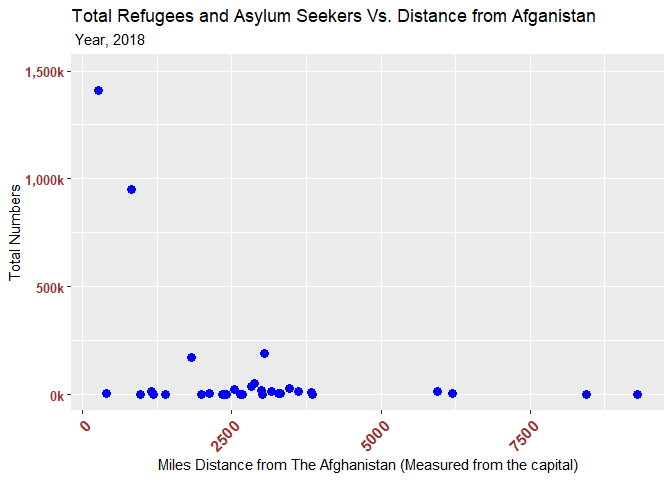
\includegraphics{Assignment-4_files/figure-latex/unnamed-chunk-15-1.pdf}

\begin{Shaded}
\begin{Highlighting}[]
\KeywordTok{plot}\NormalTok{(data_nona}\OperatorTok{$}\NormalTok{Sal[}\DecValTok{800}\OperatorTok{:}\DecValTok{950}\NormalTok{], }\DataTypeTok{main =} \StringTok{"Salinity data"}\NormalTok{)}
\KeywordTok{lines}\NormalTok{(}\KeywordTok{ts}\NormalTok{(fkf.obj1}\OperatorTok{$}\NormalTok{att[}\DecValTok{1}\NormalTok{, ], }\DataTypeTok{start =} \KeywordTok{start}\NormalTok{(y), }\DataTypeTok{frequency =} \KeywordTok{frequency}\NormalTok{(y)), }\DataTypeTok{col =} \StringTok{"blue"}\NormalTok{)}
\end{Highlighting}
\end{Shaded}

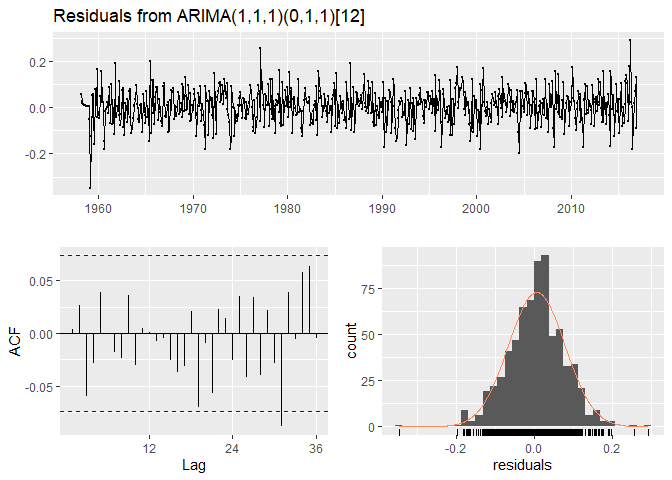
\includegraphics{Assignment-4_files/figure-latex/unnamed-chunk-16-1.pdf}


\end{document}
